% !TEX TS-program = pdflatex
% !TEX encoding = UTF-8 Unicode

% This is a simple template for a LaTeX document using the "article" class.
% See "book", "report", "letter" for other types of document.

\documentclass[11pt]{article} % use larger type; default would be 10pt

\usepackage[utf8]{inputenc} % set input encoding (not needed with XeLaTeX)

\usepackage{amssymb,amsmath}
\usepackage{graphicx}
\usepackage{caption}
\usepackage{subcaption}

%%% Examples of Article customizations
% These packages are optional, depending whether you want the features they provide.
% See the LaTeX Companion or other references for full information.

%%% PAGE DIMENSIONS
\usepackage{geometry} % to change the page dimensions
\geometry{a4paper} % or letterpaper (US) or a5paper or....
% \geometry{margin=2in} % for example, change the margins to 2 inches all round
% \geometry{landscape} % set up the page for landscape
%   read geometry.pdf for detailed page layout information

\usepackage{graphicx} % support the \includegraphics command and options

% \usepackage[parfill]{parskip} % Activate to begin paragraphs with an empty line rather than an indent

%%% PACKAGES
\usepackage{booktabs} % for much better looking tables
\usepackage{array} % for better arrays (eg matrices) in maths
\usepackage{paralist} % very flexible & customisable lists (eg. enumerate/itemize, etc.)
\usepackage{verbatim} % adds environment for commenting out blocks of text & for better verbatim
\usepackage{subfig} % make it possible to include more than one captioned figure/table in a single float
% These packages are all incorporated in the memoir class to one degree or another...

%%% HEADERS & FOOTERS
\usepackage{fancyhdr} % This should be set AFTER setting up the page geometry
\pagestyle{fancy} % options: empty , plain , fancy
\renewcommand{\headrulewidth}{0pt} % customise the layout...
\lhead{}\chead{}\rhead{}
\lfoot{}\cfoot{\thepage}\rfoot{}

%%% SECTION TITLE APPEARANCE
\usepackage{sectsty}
\allsectionsfont{\sffamily\mdseries\upshape} % (See the fntguide.pdf for font help)
% (This matches ConTeXt defaults)

%%% ToC (table of contents) APPEARANCE
\usepackage[nottoc,notlof,notlot]{tocbibind} % Put the bibliography in the ToC
\usepackage[titles,subfigure]{tocloft} % Alter the style of the Table of Contents
\renewcommand{\cftsecfont}{\rmfamily\mdseries\upshape}
\renewcommand{\cftsecpagefont}{\rmfamily\mdseries\upshape} % No bold!


%%% END Article customizations

%%% The "real" document content comes below...

\title{Super Awesome Parallel Work}
\author{Aaron Mininger and James Kirk}
%\date{} % Activate to display a given date or no date (if empty),
         % otherwise the current date is printed 



\begin{document}
\maketitle

\section{Introduction}
This paper focuses on the parallelization of episodic memory; particularly the
episodic memory mechanism in Soar: a general cognitive architecture used and
developed at Michigan by John Laird and his students. The purpose of Soar is to
support the capabilities required of a generally intelligent agent by providing
mechanisms for that agent to use. One of those mechanisms is episodic memory,
which captures snapshots or episodes of the agent’s state (working memory)
through time and stores them for later retrievals. The agent can then construct
a cue to use to search through episodic memory and find an episode that matches.

\subsection{Motivation and Challenges}
The main motivation for our project is to speedup up the time it takes to search 
through episodic memory by parallelizing this process. An important requirement
for agents that are situated in a dynamic environment is for them to be reactive, 
which means that each decision cycle
should be as quick as possible. This places very strict constraints on the
efficiency of any memories to be utilized. The current implementation of Soar’s
episodic memory has a number of efficient ways of performing a retrieval. However,
in the worst case (the cue does not have a match or only matches the oldest
episode) a search must be done through all of the episodes, which can be quite a
large number as the lifetime of the agent increases. By parallelizing episodic memory,
we aim to extend the viable lifetime of agents that use it. 
 
There are many challenges to implementing a parallel version of this mechanism.
 When a retrieval happens it must search over N episodes, but N is constantly 
increasing, likely every decision cycle. Each time a new episode is added, the 
episodes need to be rebalanced, but in an efficient manner without substantial 
amounts of shuffling and messaging and without disturbing the strict ordering
 of episodes. Any load balancing must not affect the reactivity of the agent; if 
the agent has to stop every once in a while and do a major rebalancing of 
its memory, this can severely harm its performance. 
Messaging time is likely to be a bottleneck, especially as the 
number of processors and episodes increase. It is also unknown if the agent is 
likely to be retrieving from recent memory, from old memory, or some mix in 
between.  Efficient load balancing strategies for such behaviors would be 
different and the episodic memory mechanism should be general enough to handle 
them all efficiently.

Another challenge, although not directly related parallelizing work, is the difficulty in 
modifying a large code base, the Soar kernel, without damaging any 
functionality and maintaining preexisting efficiencies.  In the serial version,
 all episode data is held in one database and needed to be split into 
smaller databases on each processor.  There was no theory for how to divide
the episode history into smaller chunks of episodes. We had to implement the ability
for a processor to remove its oldest episode and pass it to the next processor. 
This turns out to be less efficient than an addition, and is one place for further improvement
of performance.

\section{Episodic Memory in Soar}
Working memory is represented as a directed (possibly cyclic) graph. It consists
of a list of working memory elements (wme’s) that represent an edge in the graph
(starting node, edge name, ending node). During the storage of the current state
of working memory as an episode, the entire graph is not saved. Instead, only
the changes from the last episode (additions or deletions) are tracked and
stored. This means that random access into the past is not a cheap operation, as
the episode needs to be reconstructed from scratch.

The two main operations of Soar’s episodic memory mechanism are storing new
episodes and retrieving the best match for a given cue. The following sections
explain in some detail how these processes were made efficient in the existing
serial version.

\subsection{Storage}
Episodic memory is stored inside an sqlite database. As mentioned before, the
working memory graph is represented as a list of edges, or wme’s. Throughout the
lifetime of the agent, individual wme’s may be added and removed a number of
times. What is stored in the database is a list of all the wme’s that have
existed in the agent’s past, plus the intervals for which they were active. The
agent determines which working memory elements have changed since the last
storage, and either ends an active interval (for deletions), or begins a new one
(for additions). This process is very efficient, since the algorithm only has to
consider currently active wme’s; the number of which remains relatively small
and constant over the agent’s lifetime.

\subsection {Retrieval}
The agent initiates a retrieval by creating a cue to search with. The cue
represents an acyclic subgraph of working memory and the goal is to find the
episode that matches that subgraph the best. The agent does a walk backwards
from the current episode and only searches those episodes that changed with
regards to the cue. It first does a surface match based on the leaves of the
cue. The leaves are considered independent, so the structure as a whole is not
unified to the episode being considered. If it finds a matching containing all
of the leaves it does a full graph match. This is expensive (NP-complete) so it
is only done when absolutely necessary.

Whenever it finds a graph match it stops the search and returns the result. This
is because results are biased by recency; if two episodes are a perfect match
the more recent one is returned. If no episode perfectly matches, then the
entire contents of memory end up being searched. Partial matches are ranked and
the highest one is returned. The ranking is calculated from the number of leaves
that match and is again biased by recency.

\section{Parallel Implementation}
Our goal in parallelizing Soar’s episodic memory was to distribute the storage
and search of episodic memory across a set of processors. Although the search
process has been heavily optimized, it still grows over time with the number of
episodes. Agents that run over hours and days are of interest to study, and
eventually the cost of using episodic memory grows too large for the agent to be
reactive. Our goal is to be able to reduce that cost by spreading it out over a
number of processors. 

We did not set out to change the behavior of episodic memory or re-implement the
algorithms underlying the storage and retrievals. These have already been
heavily optimized and tuned for performance and any work on our part would have
had marginal effects. 

The basic structure of our implementation is as follows. The first processor runs
the Soar agent as normal. The second processor is a manager processor which 
handles requests from the agent and distribute work to the worker processors. 
There must be at least one worker, and thus at least three processors. The actual
stored episodes are spread out among the workers according to various distributions
that will be discussed later. The following
sections describe how the episodes are stored and retrieved on each worker.

\subsubsection{Storage}

Each worker has its own database that contains some window or subinterval of the agent's history. 
The workers form a chain from lowest to highest, with more recent episodes at the 
lower processors and the oldest episodes at the highest ones. No two workers have
overlapping windows, and taken all together they form the entire history. 
This window's size can be adjusted per worker dynamically as
the agent accumulates new episodes and conducts queries of episodic memory. 
When a worker hits its cap of episodes, it will generate an episode-diff structure
from its local database and send it to its immediate neighbor down the chain, 
which will then add the episode. The last worker in the chain will not remove any episodes. 

When the agent creates another episode, this new episode is sent to the
manager. The manager notifies all worker processors that it has received a new
episode. If the worker has an episode to send (meaning that it contains at least
as many episodes as its window size), it will immediately send it to its neighbor. 
The first worker processor then receives the new episode from the manager. 
Thus every worker does one send and one receive, and those do not depend
on the other processors. This prevents a linear problem that occurred on the
first implementation of episode addition. If the addition of a new episode needs
to propagate down the entire chain, the last worker has to wait potentially O(p) time, 
where p is the number of processors. Removing an episode is an expensive operation, 
so this linear delay was signficant. By having each worker make a local decision
about whether to send to the next, we sped up episode storage dramatically. 


\subsection{Retrieval}
When the agent wants to retrieve an episode it sends this request and the cue in
a message to the manager. The manager broadcasts the search request message to
all worker processes. Once a worker receives a search request it performs an
identical search algorithm as done in the serial version, only on its local portion
of the history. Each worker will return its best match, if it
has a match, in a message to the manager.

The manager selects the best episode matching from the responses. If it receives
a response that is better than any it could possibly receive from the workers it
is still waiting on, such as getting a full graph match on the first worker, the
manager will immediately send this response back to the agent. As is done in the
serial version, the manager selects the best match based on, in order of
importance, full graph matching, the match score, and if a tie recency. The
division of episodes ensures that if a worker processor has a lower id than
another, it episodes will always be more recent.

\subsection{Dynamic Load Balancing}

The window size of each worker determines the overall load balancing of the
retrieval process. The window size does not need to be fixed, and as we are
continuously adding episodes, we can increase the window size for each agent to
scale with the number of episodes. There are a few different window size scaling
strategies that could be beneficial for different agent behaviors.

The most basic scaling strategy just keeps an even split of the data among the
processors. If all episodes will need to be searched, as in the worst case, then
this will be the best load balancing. Based on the number of episodes a worker
has received it can calculate when it needs to increase its window size without
messaging any other processors. The equation for determining if the window size
needs to be increased is shown below in equation 1.

\begin{equation}
incrWindow? = ((count  \bmod  (2^{(P-i)} -1) ) == 0)
\end{equation}

The $count$ is the total number of episodes this worker has received, $P$ is the
number of processors, and $i$ is the id of the worker processor. Every time the
worker has received another $ 2^(P-i) -1 $ episodes it should increment its window
size by 1.

Another strategy is to have the size of the window increase exponential from the
first worker to the last worker, which holds the oldest episodes. For example
for a small case with 5 workers and 310 episodes added so far, the workers would
hold in order for youngest to oldest, 10, 20, 40, 80, and 160 episodes. This
compares to the above strategy where each worker would hold 62 episodes. If the
agent is always retrieving recent episode this will likely be an improvement
from the previous strategy. In this case if the matching episode is in the first
70 episodes, the exponential window size strategy will likely finish before an
even window strategy. Similar to the equation for the previous strategy, the
worker can determine when to increase its window size.

\begin{equation}incrWindow? = ((count  \bmod  (P-i) ) == 0)\label{eq.1}\end{equation}

However, the idea of Soar is to have general purpose mechanisms like episodic
memory that are useful for agents. When developing an agent, there should not be
required changes to the kernel to select the best episodic memory behavior.
Additionally we should not require agent developers to characterize their
episodic memory retrievals, whether they are mostly in recent memory or older
memory or some mix. Even with a given agent this behavior could differ depending
on the situation the agent is in.

To address this situation a third strategy was developed to split the difference
between the above strategies and to dynamically alter behavior based on
retrievals. The difference between above strategies number of episodes received
before a window size increase, $2^(P-i) -1$ in the first case and $P-i$ in the
second case. In the dynamic version we select a value between these two by means
of a split variable between 0 and 1.0. The equations for this algorithm can be
seen below.

\begin{equation}x = (2^(P-i) -1)*split + (P-i) *(1-split)\end{equation}
\begin{equation}incrWindow? = ((count \bmod x) == 0)\end{equation}

The value of split is initially set to 0.5, splitting the difference evenly so
that the episode allocation is not even, but also less than exponential in
increase. Every time a retrieval occurs, the worker episode that returned the
best result is used to update the split value, a global value the is calculated
by the manager and broadcast to all workers. An update split value can be
calculated by the percentile that the best response came from. If the best
response comes from the earliest worker, processor 2, the update value will be
1, and if from the oldest worker the update value will be 0. The split value is
averaged with this update value using a tuning parameter. If the parameter is
0.5 then the update value contributes to half of the new split value. In
experimentation this parameter was varied over a few different values to see the
effect on window size growth and distribution.

\section{Experimental Results}
This section describes our experimental process and how data was collected. 
It also includes the presentation of the data and a discussion of its interpretation. 

\subsection{Evaluation Methodology}
Thorougly testing episodic memory is a challenging task, because there are a number
of factors that can influence performance. Such factors include the number of processors,
the type of agent, the agent's environment and working memory,  the types of queries the agent performs,
 how long the agent has been running, and how the episodes are distributed. 

For all our tests, we compared the performance using different numbers of processors
ranging from 1-32 by powers of two. This allowed us to get an estimation of the speedup
achieved by the program. In addition, for some of the trials we compared against two 
baseline versions. The one is an unmodified version of episodic memory (denoted UM) and
the other is one with our modifications, but with everything happening on a single processor 
(denoted ST). 

Every agent is different, and each one has a different working memory and a different
use pattern for episodic memory. We thus did not try to evaluate across different agents, 
but instead desired to characterize the types of retrievals an agent could do and how those
affect performance. For our agent we could specify an interval of where to do retrievals 
in, and how often it does a retrieval. 
\emph{Long retrievals} are those that either don't result in a graph match, or 
result in an episode at the beginning of episodic memory. In those cases the agent has to 
search through all the episodes. For this case the agent produces cues that resulted
in episodes randomly within the first tenth of its history. \emph{Short retrievals} are those
that result in a full graph match within the lastest tenth of its history. For this case the agent produces 
cues that resulted in an episode about ten percent back in its history. \emph{Random retrievals} are
those that result in a full graph match at a random episode in its history. 

For all of the agents, the retrievals and episode creation were setup as
follows. At every time step the agent adds and removes elements from working
memory, which will cause the addition of a new episode to episodic memory. Every
1,000 times steps, or 1,000 episodes, the agent issues an epmem query. The type of
query is dependent upon the particular test. The time is captured from right before the agent sends the query
message, to when the agent receives the response. The serial timing is captured
similarly, starting after the construction of the cue, and ending when a
response is found.

As well as doing a retrieval every 1000 time steps, the timing of episode
storage is recorded every 1001 time steps. The offset is used so that a good
representation of episode addition times is collected. We noticed during testing
that some parallel episode storages take significantly longer than others. This
is due to some storages not requiring any old episode removals, i.e. every worker
is not full or not receiving a new episode. When there are only 2 workers, every
other episode addition is quicker. The offset ensures that we get an even
sampling of the addition times for comparison.

We also ran tests with different episode distribution strategies. An \emph{even strategy} was
where the episodes were distributed evenly across the processors. This was designed to
improve performance for agents that only do long retrievals. A \emph{shift strategy} was
where the first $p-1$ workers were evenly distributed across the first $20\%$ of the episodes, and 
the last worker has the rest. This was designed to improve performance for agents that only do
short retrievals. A \emph{dynamic strategy} was a mixture of the two, where the proportion of the 
history stored by the last worker would dynamically increase or decrease depending on the particular
kinds of queries being executed. 


\subsection{Long Retrievals}
Our first trial was to cover the worst case in retrieval time: when the episode is at the beginning of 
the agent's history or there are no exact matches. In this case the agent must search through all 
the episodes to find the one to return. This represents the greatest opportunity for us to take advantage 
of the parallelism. For this test we had the agent retrieve episodes in the first ten percent of its history. 
We also varied the number of worker processors from 1 to 32 and compared the results with the unmodified 
Soar version (UM) and a version with our modifications but with everything running on a single thread (ST). 

\begin{figure}
        \centering
        \begin{subfigure}[b]{0.55\textwidth}
                \centering
                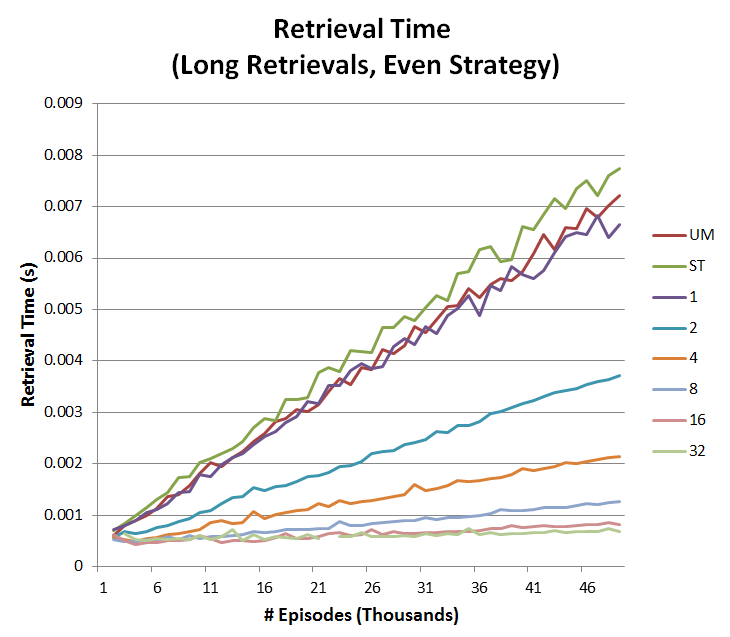
\includegraphics[width=\textwidth]{images/ret_long_eq}
                \label{fig:retleq}
        \end{subfigure}%
        ~ %add desired spacing between images, e. g. ~, \quad, \qquad etc. 
          %(or a blank line to force the subfigure onto a new line)
        \begin{subfigure}[b]{0.55\textwidth}
                \centering
                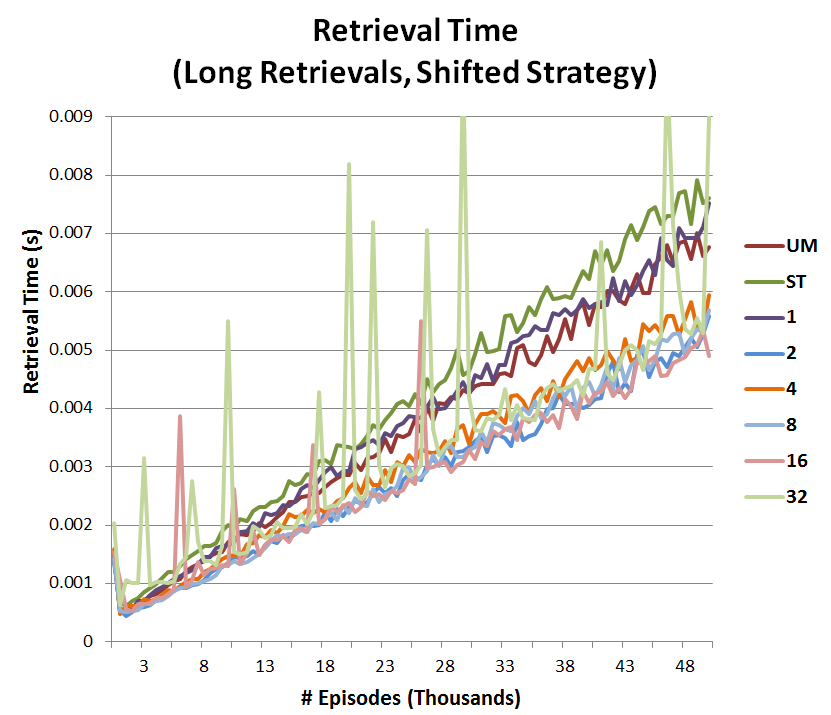
\includegraphics[width=\textwidth]{images/ret_long_shift}
                \label{fig:retlexp}
        \end{subfigure}
        \caption{Running time for long retrievals}\label{fig:animals}
	\label{fig:long}
\end{figure}

The results as shown in figure \ref{fig:long} show that our version with 1 worker performs as well as the unmodified Soar version (UM). 
This gives good support that our modifications have not slowed down the retrieval processes in the serialized case. 
The single thread (ST) case was a bit slower than the case with 1 worker, but it has to manage two databases on the same processor. 
The retrieval time shows linear growth with the number of episodes 
as expected, since the agent has to search linearly through all of the episodes to find a match. 
For the results on the left with an even distribution strategy, we get an improvement of performance until about 16 processors. 
This case represents the greatest possibility for speedup because all the episodes need to be searched, and they are distributed evenly 
among the processors. For the results on the right with a shifted distribution strategy, there is no benefit to having more than 2 workers.
This is because $80\%$ of the episodes are being stored on the last processor. This is as expected, the shifted strategy does poorly for 
queries with long retrieval times. 


\subsection{Short Retrievals}
Our next trial was to cover short retrievals: when the cue matches a recent episode.  
If the episode is at the very end of the history, then the retrieval time will be constant and parallelization 
won't do any good. We thus examined where the agent was searching about a tenth back through its history. 
This range still makes parallelization a challenge, but it is possible to get some net benefit. 

\begin{figure}
        \centering
        \begin{subfigure}[b]{0.55\textwidth}
                \centering
                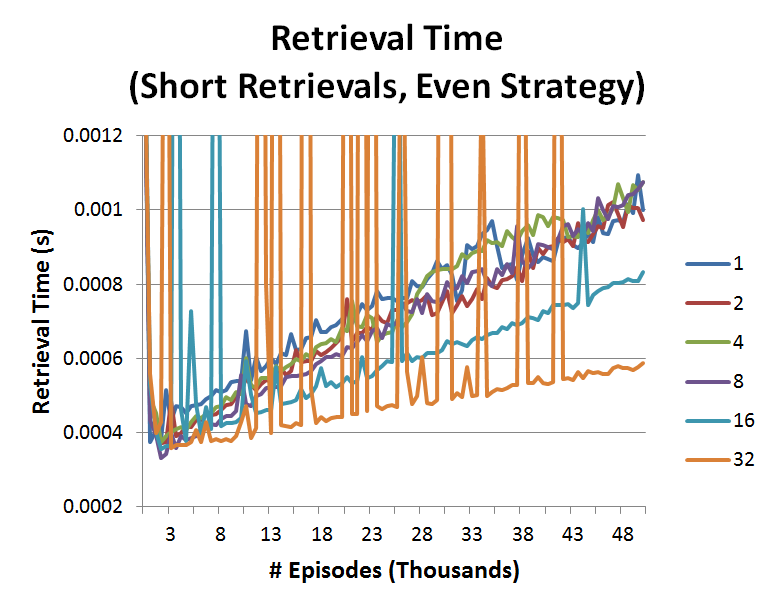
\includegraphics[width=\textwidth]{images/ret_short_eq}
                \label{fig:retseq}
        \end{subfigure}%
        ~ %add desired spacing between images, e. g. ~, \quad, \qquad etc. 
          %(or a blank line to force the subfigure onto a new line)
        \begin{subfigure}[b]{0.55\textwidth}
                \centering
                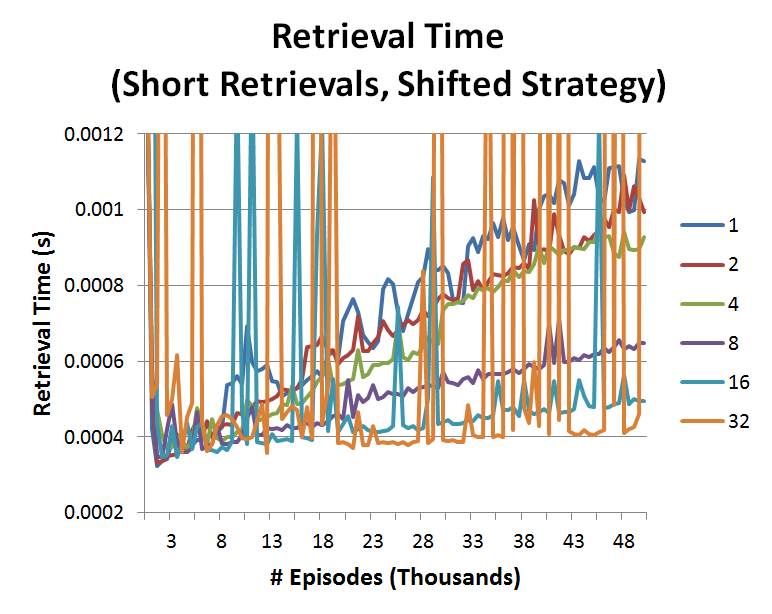
\includegraphics[width=\textwidth]{images/ret_short_shift}
                \label{fig:retsshift}
        \end{subfigure}
        \caption{Running time for short retrievals}
	\label{fig:short}
\end{figure}

The results as shown in figure \ref{fig:short} show that indeed it is hard to parallelize short retrievals. As long as the episode is within the window 
of the first processor (which occurs up through 8 processors) there is no benefit to having it parallelized. 

our version with 1 worker performs as well as the unmodified Soar version (UM). 
This gives good support that our modifications have not slowed down the retrieval processes in the serialized case. 
The single thread (ST) case was a bit slower than the case with 1 worker, but it has to manage two databases on the same processor. 
The retrieval time shows linear growth with the number of episodes 
as expected, since the agent has to search linearly through all of the episodes to find a match. 
For the results on the left with an even distribution strategy, we get an improvement of performance until about 16 processors. 
This case represents the greatest possibility for speedup because all the episodes need to be searched, and they are distributed evenly 
among the processors. For the results on the right with a shifted distribution strategy, there is no benefit to having more than 2 workers.
This is because $80\%$ of the episodes are being stored on the last processor. This is as expected, the shifted strategy does poorly for 
queries with long retrieval times. 

\subsection{Random Retrievals}
Description of the test case
\begin{figure}[h]
\caption{Results for random retrievals and equal episode distribution}
\centering
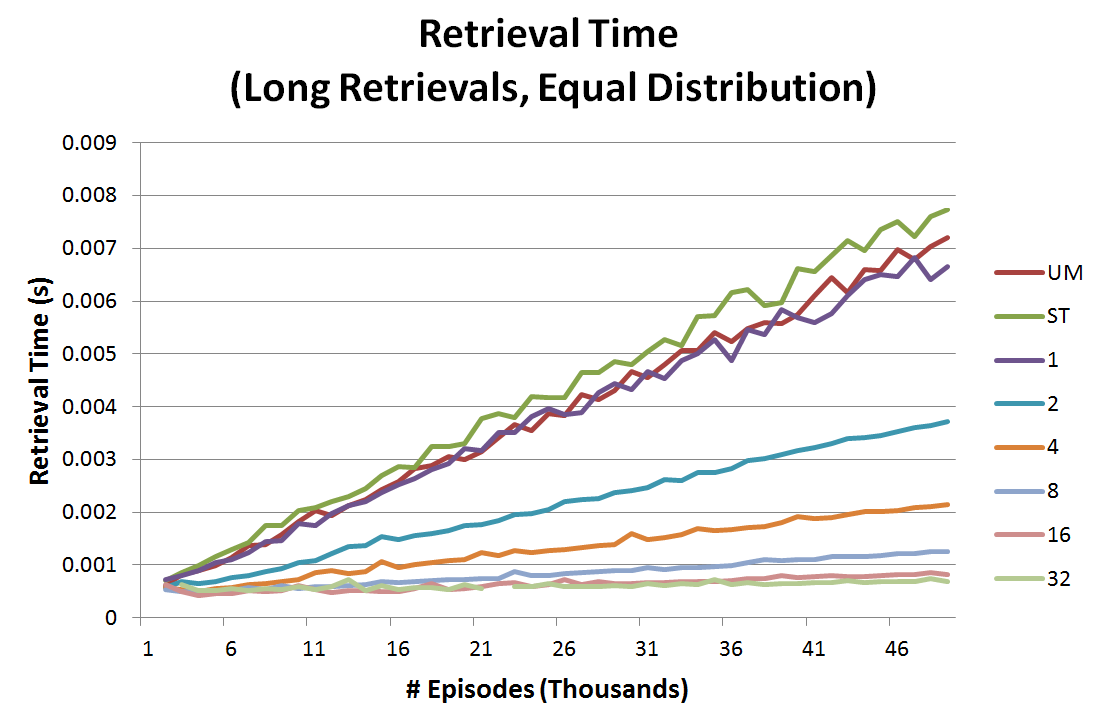
\includegraphics[width=0.75\textwidth]{images/ret_worst_eq}
\end{figure}

\begin{figure}[h]
\caption{Results for random retrievals and exponential episode distribution}
\centering
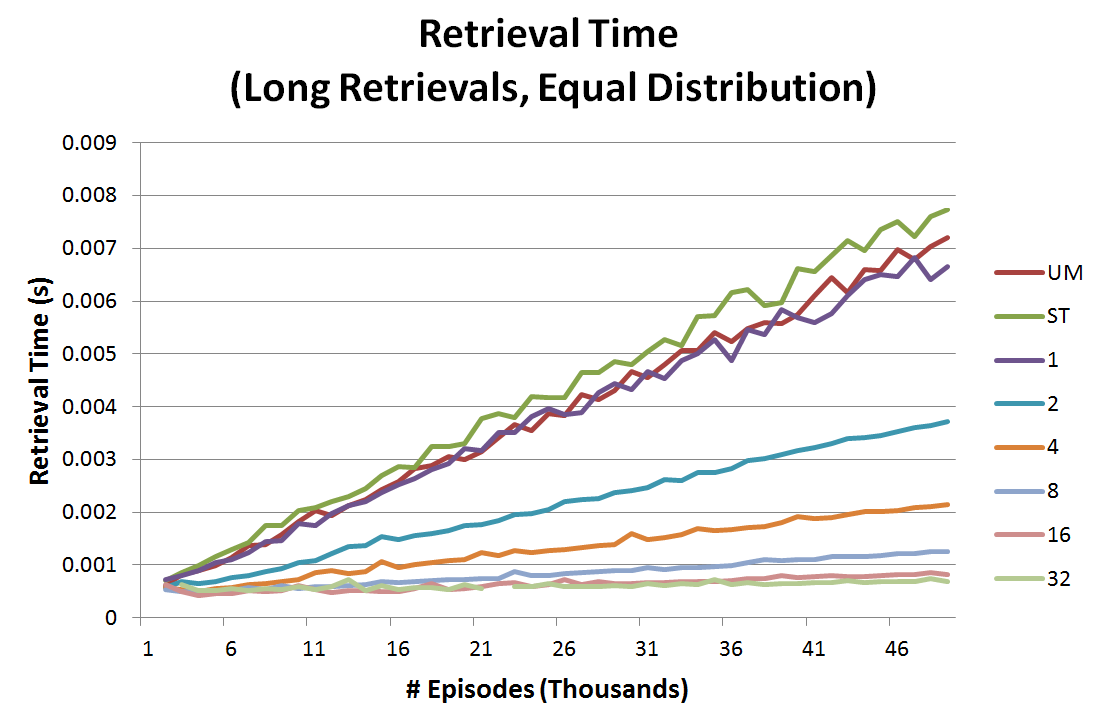
\includegraphics[width=0.75\textwidth]{images/ret_worst_eq}
\end{figure}

\subsection{Dynamic Partitioning}
Description of the modifications
\begin{figure}[h]
\caption{Histogram with long retrievals}
\centering
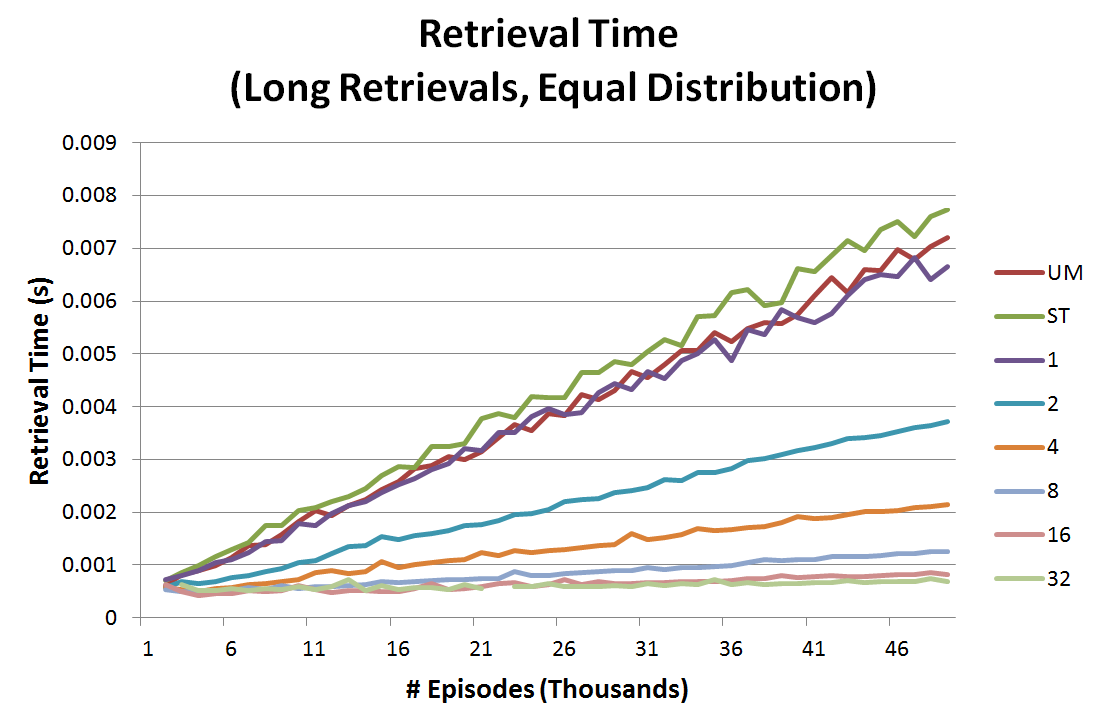
\includegraphics[width=0.75\textwidth]{images/ret_worst_eq}
\end{figure}

\begin{figure}[h]
\caption{Histogram with short retrievals}
\centering
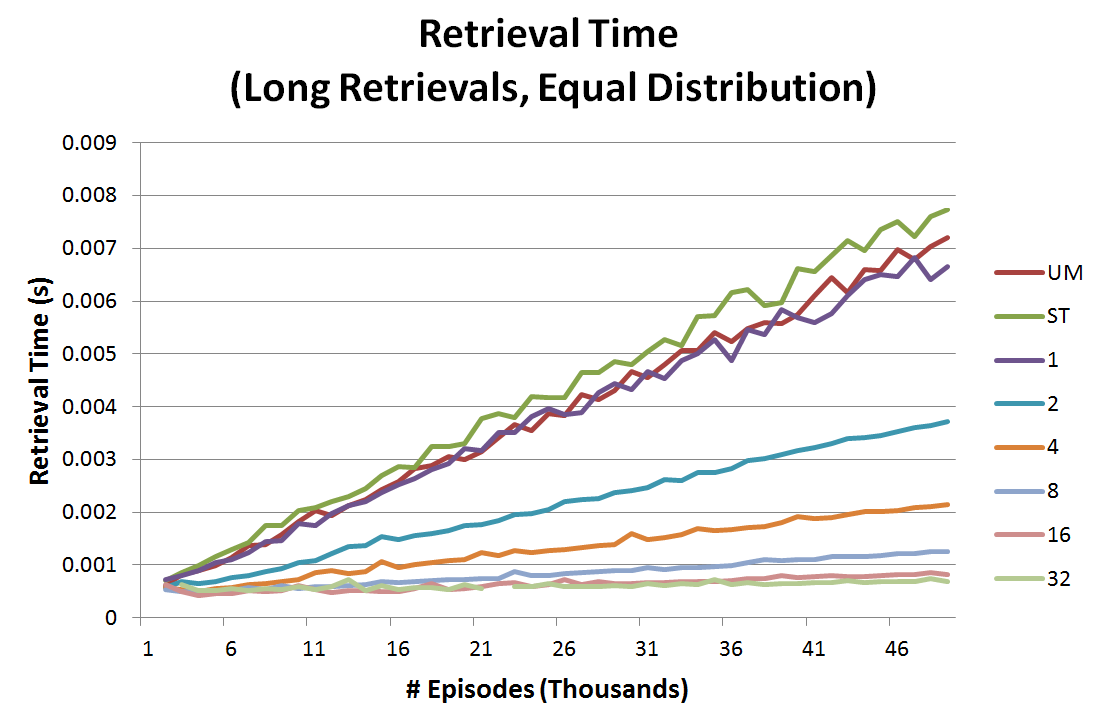
\includegraphics[width=0.75\textwidth]{images/ret_worst_eq}
\end{figure}

\begin{figure}[h]
\caption{Histogram with random retrievals}
\centering
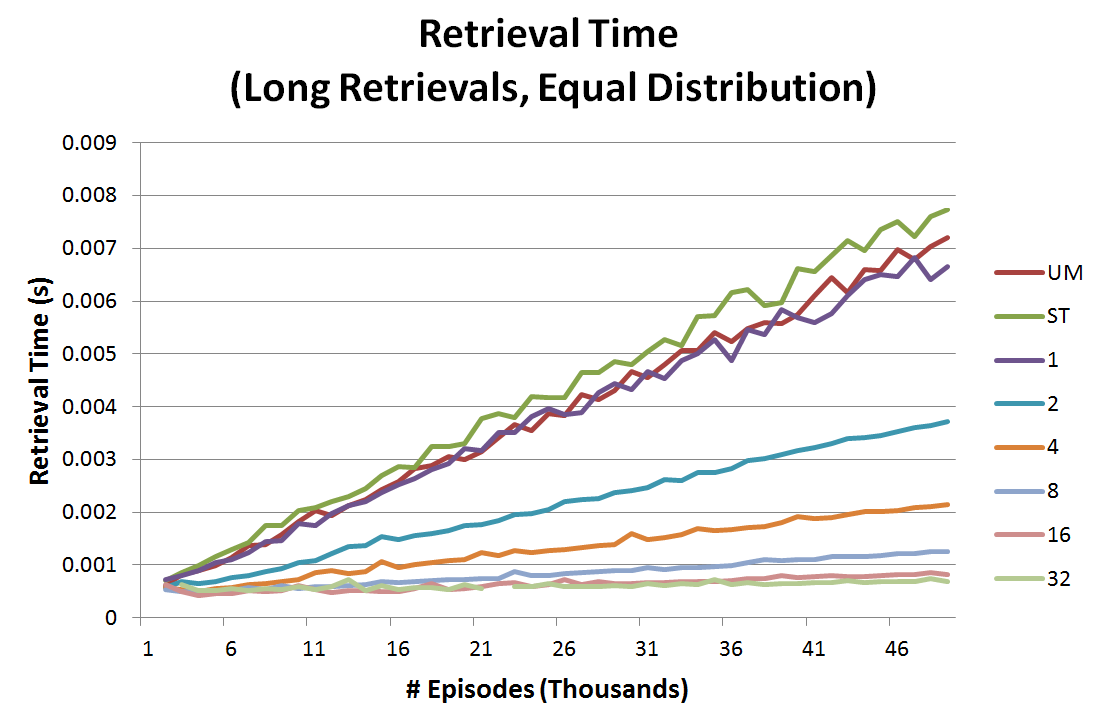
\includegraphics[width=0.75\textwidth]{images/ret_worst_eq}
\end{figure}

Discussion of histograms

\begin{figure}[h]
\caption{Performance for short retrievals and parameter tuning}
\centering
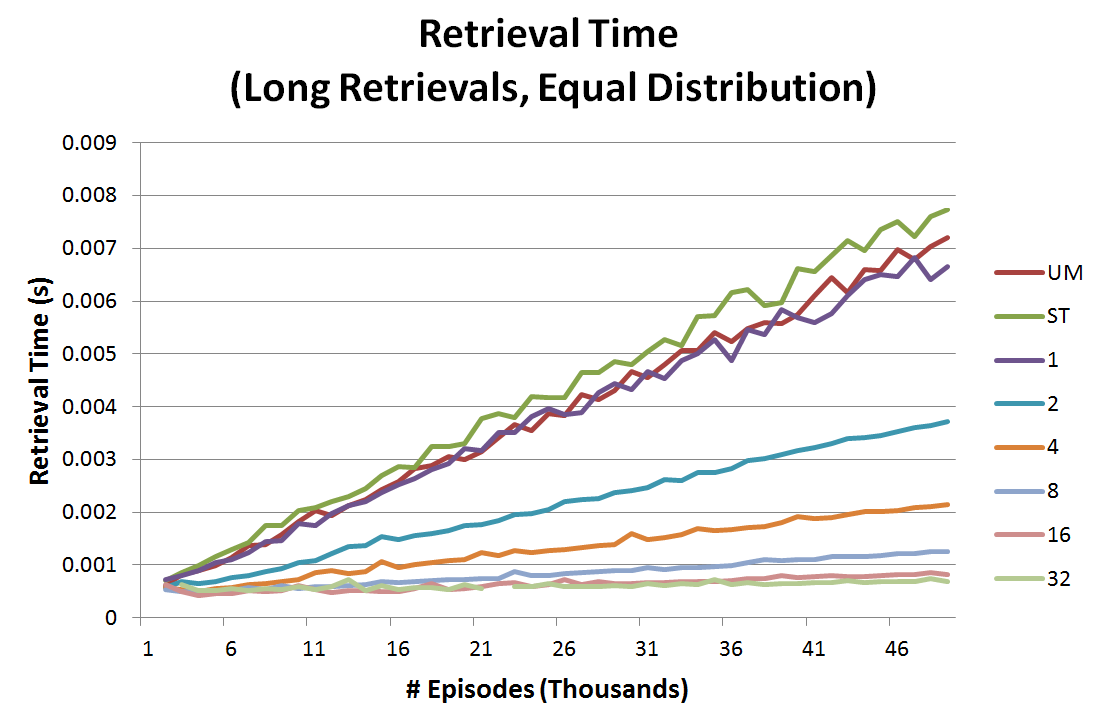
\includegraphics[width=0.75\textwidth]{images/ret_worst_eq}
\end{figure}

\begin{figure}[h]
\caption{Performance for random retrievals and parameter tuning}
\centering
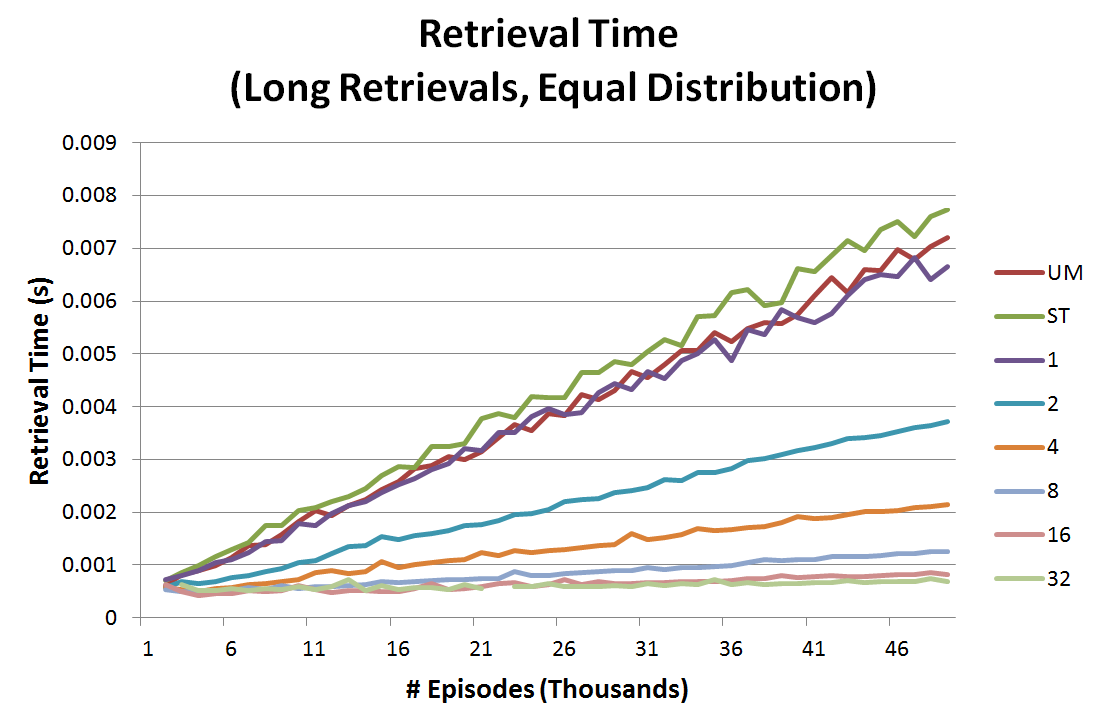
\includegraphics[width=0.75\textwidth]{images/ret_worst_eq}
\end{figure}

Discussion of results

\begin{table}[h]
\caption{Table of speedup}
\centering
    \begin{tabular}{|l|r|r|r|r|r|r|r|r|r|}
        \hline
        ~  & Equal Long & Equal Short & Equal Rand & Exp Long & Exp Short & Exp Rand & Dyn Long & Dyn Short & Dyn Rand \\ \hline
        1  & ~          & ~           & ~          & ~        & ~         & ~        & ~        & ~         & ~        \\  \hline
        2  & ~          & ~           & ~          & ~        & ~         & ~        & ~        & ~         & ~        \\ \hline
        4  & ~          & ~           & ~          & ~        & ~         & ~        & ~        & ~         & ~        \\ \hline
        8  & ~          & ~           & ~          & ~        & ~         & ~        & ~        & ~         & ~        \\ \hline
        16 & ~          & ~           & ~          & ~        & ~         & ~        & ~        & ~         & ~        \\ \hline
        32 & ~          & ~           & ~          & ~        & ~         & ~        & ~        & ~         & ~        \\
        \hline
    \end{tabular}
\end{table}

\subsection{Storage}

What's going on with storage

\begin{figure}[h]
\caption{Comparison of Storing times}
\centering
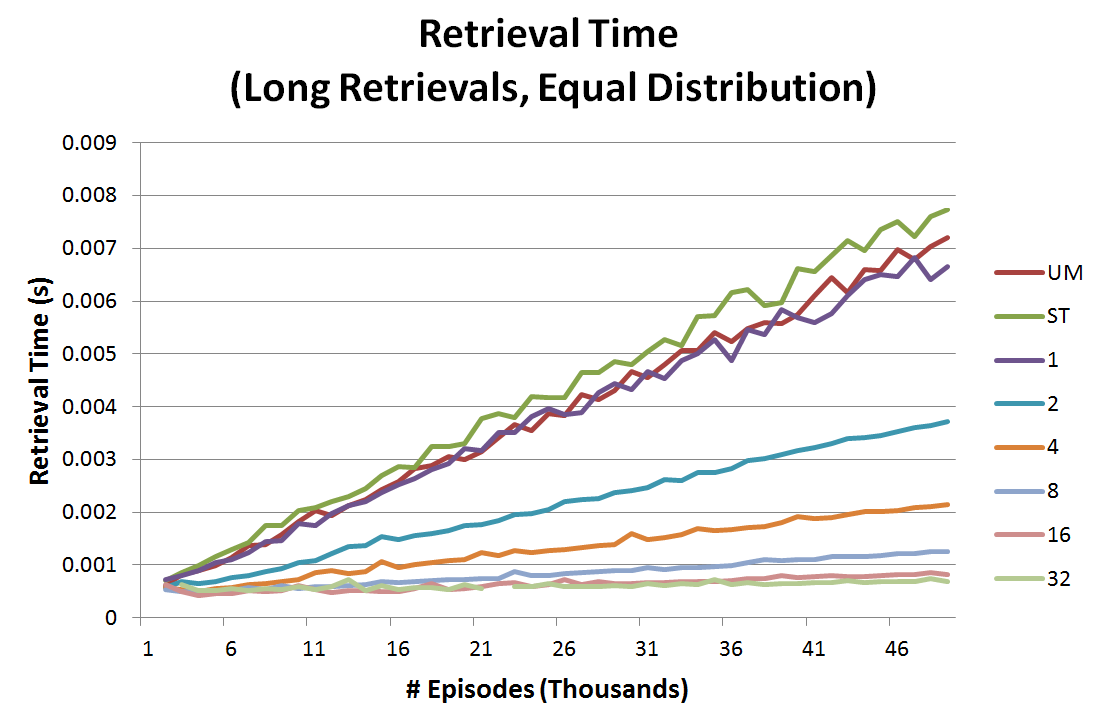
\includegraphics[width=0.75\textwidth]{images/ret_worst_eq}
\end{figure}

Description of results


\section{Conclusions}

\section{References}

Derbinsky, N., and Laird, J. E. (2009). Efficiently Implementing Episodic
Memory. Proceedings of the International Conference on Case-based Reasoning.



\end{document}
